\section{图的连通性}
\begin{definition}
%@see: 《离散数学》(邓辉文) P177 定义6-16
设图\(G = (V,E)\).
若从顶点\(u\)到\(v\)之间存在一条路,
则称“\(u\) \DefineConcept{可达} \(v\)”.
\end{definition}

由于任意一个顶点\(v\)到它自己之间总存在一条平凡路,
因此每一个顶点均可达它自己.

\begin{definition}
设图\(G = (V,E)\).
若\(u\)可达\(v\),且\(v\)可达\(u\),
则称“\(u\)和\(v\) \DefineConcept{相互可达}”.
\end{definition}

\subsection{无向图的连通性}
\begin{definition}
%@see: 《离散数学》(邓辉文) P177 定义6-17
设无向图\(G = (V,E)\).
如果对于任意两个顶点\(u,v \in V\),
\(u\)可达\(v\),
则称“\(G\)是一个\DefineConcept{连通图}(connected graph)”.
\end{definition}

\begin{definition}
%@see: 《离散数学》(邓辉文) P178 定义6-18
无向图\(G\)中极大的连通子图
称为“\(G\)的一个\DefineConcept{连通分量}(connected component)”.
\end{definition}

\begin{definition}
%@see: 《离散数学》(邓辉文) P178 定义6-18
无向图\(G = (V,E)\)的连通分量个数记为\(w(G)\).
\end{definition}

\begin{theorem}
%@see: 《离散数学》(邓辉文) P178 定理6-4
设无向图\(G = (V,E)\),
则\[
	\text{$G$是连通图}
	\iff
	w(G) = 1.
\]
\end{theorem}

\begin{corollary}
%@see: 《离散数学》(邓辉文) P178
设无向图\(G = (V,E)\),
则\[
	\text{$G$是非连通图}
	\iff
	w(G) \geq 2.
\]
\end{corollary}

\begin{example}
%@see: 《离散数学》(邓辉文) P178 例6-5
设\(G = (V,E)\)是简单无向图.
若\(G\)不是连通图,
则\(G\)的补图\(\overline{G}\)是连通图.
%TODO proof
\end{example}

\begin{example}
%@see: 《离散数学》(邓辉文) P178 例6-6
设\(G = (V,E)\)是\(n\)阶简单无向图.
证明:若\[
	(\forall u,v \in V)
	\left[
		\text{$u,v$不邻接}
		\implies
		\deg u + \deg v \geq n - 1
	\right],
\]
则\(G\)是连通图.
%TODO proof
\end{example}

\begin{theorem}
%@see: 《离散数学》(邓辉文) P178 定理6-5
设\(G = (V,E)\)是连通无向图,则\begin{itemize}
	\item 去掉\(G\)中任意简单回路\(C\)上的一条边\(e\)得到的图\(G - e\)还是连通图;
	\item 去掉一个度数为1的顶点\(v\)得到的图\(G - v\)还是连通图.
\end{itemize}
%TODO proof
\end{theorem}

\subsection{连通无向图的点连通度}
不同的连通无向图的连通的“程度”是各不相同的,有的图的连通性很“脆弱”,有的则与之相反.

\begin{definition}
%@see: 《离散数学》(邓辉文) P178 定义6-19
设\(G = (V,E)\)是连通无向图,且\(W \subset V\).
若\begin{itemize}
	\item 从\(G\)中删除\(W\)的所有顶点所得到的子图\(G-W\)不是连通图,或者\(G-W\)是1阶图,
	\item 而且删除\(W\)的任意一个真子集所得到的子图都还是连通图,
\end{itemize}
则称“\(W\)是\(G\)的\DefineConcept{点割集}(cut-set of vertices)”.

特别地,如果\(G\)的点割集是一个单元素集\(W = \{v\}\),
则称“\(v\)是\(G\)的\DefineConcept{割点}(cut point)”
或“\(v\)是\(G\)的\DefineConcept{关节点}(articulation point)”.
\end{definition}

由定义可知,1阶图的点割集为\(\emptyset\).
在\cref{figure:图论.点割集1} 中,图的点割集是\(\{a,b\},\{c,d\}\).

\begin{figure}[hbt]
%@see: 《离散数学》(邓辉文) P179 图6-27(a)
	\centering
	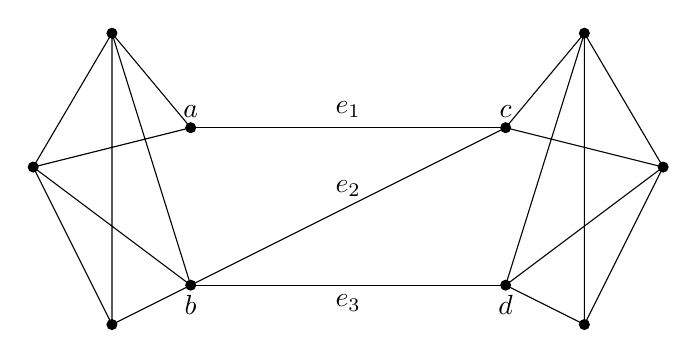
\begin{tikzpicture}
		\fill(0,0)coordinate(a)node[above]{$a$}circle(2pt);
		\fill(0,-2)coordinate(b)node[below]{$b$}circle(2pt);
		\fill(4,0)coordinate(c)node[above]{$c$}circle(2pt);
		\fill(4,-2)coordinate(d)node[below]{$d$}circle(2pt);
		\fill(-1,1.2)coordinate(v1)circle(2pt);
		\fill(-2,-.5)coordinate(v2)circle(2pt);
		\fill(-1,-2.5)coordinate(v3)circle(2pt);
		\fill(5,1.2)coordinate(u1)circle(2pt);
		\fill(6,-.5)coordinate(u2)circle(2pt);
		\fill(5,-2.5)coordinate(u3)circle(2pt);
		\draw(a)--(c)node[midway,above]{$e_1$};
		\draw(b)--(c)node[midway,above]{$e_2$};
		\draw(b)--(d)node[midway,below]{$e_3$};
		\draw(v1)--(a) (v1)--(v2) (v1)--(v3) (v1)--(b) (v2)--(a) (v2)--(b) (v2)--(v3) (v3)--(b);
		\draw(u1)--(c) (u1)--(u2) (u1)--(u3) (u1)--(d) (u2)--(c) (u2)--(d) (u2)--(u3) (u3)--(d);
	\end{tikzpicture}
	\caption{}
	\label{figure:图论.点割集1}
\end{figure}

\begin{definition}
%@see: 《离散数学》(邓辉文) P179 定义6-20
设\(G = (V,E)\)是连通无向图.
把\[
	\min\Set{
		\abs{W}
		\given
		\text{$W$是$G$的点割集}
	}
\]称为\(G\)的\DefineConcept{点连通度}(vertex-connectivity),
记作\(\kappa(G)\).
\end{definition}

根据定义,一个连通无向图\(G\)的点连通度是,
使\(G\)成为非连通图,
或使\(G\)成为1阶图,
所要删去的最少的顶点数.
于是,1阶图的点连通度为0,
而\(n\)阶完全无向图\(K_n\)的点连通度为\(\kappa(K_n) = n-1\).

在\cref{figure:图论.点割集1} 中,图的点连通度为\(2\).

\subsection{连通无向图的边连通度}
\begin{definition}
%@see: 《离散数学》(邓辉文) P179 定义6-21
设\(G = (V,E)\)是连通无向图,\(F \subset E\).
若\begin{itemize}
	\item 从\(G\)中删除\(F\)的所有边所得到的子图\(G-F\)不是连通图,或者\(G-F\)是平凡图,
	\item 而且删除\(F\)的任意一个真子集所得到的子图都还是连通图,
\end{itemize}
则称“\(F\)是\(G\)的\DefineConcept{边割集}(cut-set of edges)”.

特别地,如果\(G\)的边割集是一个单元素集\(F = \{e\}\),
则称“\(e\)是\(G\)的\DefineConcept{割边}”
或“\(e\)是\(G\)的\DefineConcept{桥}(bridge)”.
\end{definition}

在\cref{figure:图论.点割集1} 中,图的边割集是\(\{e_1,e_2,e_3\}\).

\begin{definition}
%@see: 《离散数学》(邓辉文) P179 定义6-22
设\(G = (V,E)\)是连通无向图.
把\[
	\min\Set{
		\abs{F}
		\given
		\text{$F$是$G$的边割集}
	}
\]称为\(G\)的\DefineConcept{边连通度}(edge-connectivity),
记作\(\lambda(G)\).
\end{definition}

根据定义,一个连通无向图\(G\)的边连通度是,
使\(G\)成为非连通图,
或使\(G\)成为平凡图,
所要删去的最少的边数.

在\cref{figure:图论.点割集1} 中,图的边连通度为\(3\).

% 下面的定理是 H. Whitney 在1932年给出的,关于点连通度、边连通度及最小度之间的联系.
\begin{theorem}
%@see: 《离散数学》(邓辉文) P179 定理6-6
设\(G\)是连通无向图,
则\(G\)的点连通度\(\kappa(G)\)、边连通度\(\lambda(G)\)及最小度\(\delta(G)\)满足\[
	\kappa(G)
	\leq
	\lambda(G)
	\leq
	\delta(G).
\]
%TODO proof
\end{theorem}

\subsection{有向图的连通性}
无向图只有连通与不连通两种情况,而有向图存在多种连通特性.

\begin{definition}
%@see: 《离散数学》(邓辉文) P180 定义6-23
设\(G = (V,E)\)是有向图.
如果\[
	(\forall u,v \in V)
	\left[
		\text{$u$和$v$相互可达}
	\right],
\]
则称“\(G\)是\DefineConcept{强连通图}(strongly connected digraph)”.
\end{definition}

\begin{figure}[hbt]
%@see: 《离散数学》(邓辉文) P180 图6-28
	\centering
	\def\subwidth{.25\linewidth}
	\begin{subfigure}[b]{\subwidth}
		\centering
		\begin{tikzpicture}
			\fill(0,0)coordinate(A1)circle(2pt)
				++(3,0)coordinate(A2)circle(2pt)
				++(0,2)coordinate(A3)circle(2pt)
				++(-3,0)coordinate(A4)circle(2pt);
			\begin{scope}[-{Latex[length=3mm,width=0pt 10]}]
				\draw(A1)--(A4);
				\draw(A4)--(A3);
				\draw(A3)--(A2);
				\draw(A2)--(A1);
			\end{scope}
		\end{tikzpicture}
		\caption{强连通图}
	\end{subfigure}~\begin{subfigure}[b]{\subwidth}
		\centering
		\begin{tikzpicture}
			\fill(0,0)coordinate(A1)circle(2pt)
				++(3,0)coordinate(A2)circle(2pt)
				++(0,2)coordinate(A3)circle(2pt)
				++(-3,0)coordinate(A4)circle(2pt);
			\begin{scope}[-{Latex[length=3mm,width=0pt 10]}]
				\draw(A1)--(A2);
				\draw(A1)--(A4);
				\draw(A4)--(A3);
				\draw(A3)--(A2);
			\end{scope}
		\end{tikzpicture}
		\caption{单向连通图}
	\end{subfigure}~\begin{subfigure}[b]{\subwidth}
		\centering
		\begin{tikzpicture}
			\fill(0,0)coordinate(A1)circle(2pt)
				++(3,0)coordinate(A2)circle(2pt)
				++(0,2)coordinate(A3)circle(2pt)
				++(-3,0)coordinate(A4)circle(2pt);
			\begin{scope}[-{Latex[length=3mm,width=0pt 10]}]
				\draw(A2)--(A1);
				\draw(A2)--(A3);
				\draw(A4)--(A1);
				\draw(A4)--(A3);
			\end{scope}
		\end{tikzpicture}
		\caption{弱连通图}
	\end{subfigure}
	\caption{}
\end{figure}

\begin{figure}[hbt]
%@see: 《离散数学》(邓辉文) P180 图6-29
	\centering
	\begin{tikzpicture}
		\fill(0,0)coordinate(v1)node[above]{1}circle(2pt)
			(-1,{-sqrt(3)})coordinate(v2)node[below]{2}circle(2pt)
			(1,{-sqrt(3)})coordinate(v3)node[below]{3}circle(2pt)
			(2,0)coordinate(v4)node[above]{4}circle(2pt)
			(3,{-sqrt(3)})coordinate(v5)node[below]{5}circle(2pt)
			(4,0)coordinate(v6)node[above]{6}circle(2pt);
		\begin{scope}[-{Latex[length=3mm,width=0pt 10]}]
			\draw(v1)--(v2);
			\draw(v2)--(v3);
			\draw(v3)--(v1);
			\draw(v1)--(v4);
			\draw(v4)--(v5);
			\draw(v6)--(v5);
		\end{scope}
	\end{tikzpicture}
	\caption{}
	\label{figure:图论.图的连通性.有向图1}
\end{figure}

\begin{theorem}
%@see: 《离散数学》(邓辉文) P180 定理6-7
设\(G = (V,E)\)是\(n\ (n\geq2)\)阶有向图,
则\(G\)是强连通图,
当且仅当\(G\)中存在一条回路,它通过所有顶点.
%TODO proof
\end{theorem}

\begin{definition}
%@see: 《离散数学》(邓辉文) P180 定义6-24
设\(G = (V,E)\)是有向图,
\(G\)的极大强连通子图
称为“\(G\)的\DefineConcept{强连通分量}(strongly connected component)”.
\end{definition}

\cref{figure:图论.图的连通性.有向图1} 所示的图\(G\)有4个强连通分量,
分别是\(G[1,2,3],G[4],G[5],G[6]\).

\begin{theorem}
%@see: 《离散数学》(邓辉文) P180 定理6-8
设\(G = (V,E)\)是有向图,
则\(G\)的任意顶点\(v \in V\)都位于且仅位于\(G\)的一个强连通分量中.
\begin{proof}
存在性.
对于任意顶点\(v \in V\),
令\[
	W \defeq \Set{ u \given \text{$u$和$v$相互可达} },
\]
则\(G[W]\)是\(G\)的一个强连通分量,且\(v\)位于\(G[W]\)中.

唯一性.
若顶点\(v\)位于两个不同的强连通分量\(C_1,C_2\)中,
则\(C_1,C_2\)中的任意顶点都相互可达,
于是得到一个更大的强连通子图,矛盾!
\end{proof}
\end{theorem}

\begin{definition}
%@see: 《离散数学》(邓辉文) P180 定义6-25
设\(G = (V,E)\)是有向图.
如果对于任意顶点\(u,v \in V\),
要么\(u\)可达\(v\),要么\(v\)可达\(u\),
则称“\(G\)是\DefineConcept{单向连通图}(unilateral connected digraph)”.
\end{definition}

\begin{theorem}
%@see: 《离散数学》(邓辉文) P181 定理6-9
设\(G = (V,E)\)是有向图,
则\(G\)是单向连通图,
当且仅当\(G\)中存在一条路,
它通过所有顶点.
%TODO proof
\end{theorem}

\begin{definition}
%@see: 《离散数学》(邓辉文) P181 定义6-26
设\(G = (V,E)\)是有向图.
\(G\)的极大单向连通子图,
称为“\(G\)的单向连通分量(unilateral connected component)”.
\end{definition}

\cref{figure:图论.图的连通性.有向图1} 所示的图\(G\)有2个单向连通分量,
分别是\(G[1,2,3,4,5],G[5,6]\).

\begin{definition}
%@see: 《离散数学》(邓辉文) P181 定义6-27
设\(G = (V,E)\)是有向图.
若\(G\)的基础图是连通无向图,
则称“\(G\)是\DefineConcept{弱连通图}(weakly connected digraph)”.
\end{definition}

强连通图一定是单向连通图,单向连通图一定是弱连通图,
但是,弱连通图不一定是单向连通图,单向连通图不一定是强连通图.

\begin{definition}
%@see: 《离散数学》(邓辉文) P181 定义6-28
设\(G = (V,E)\)是有向图.
\(G\)的极大弱连通子图,
称为“\(G\)的\DefineConcept{弱连通分量}(weakly connected component)”.
\end{definition}
